\chapter{Sviluppo del Software}

\section{Strumenti e tecnologie}

Lo sviluppo del software prevede tre componenti principali: il firmware per i dispositivi
embedded, il server federato e l'interfaccia utente.

Per ognuno di questi elementi sono stati utilizzati strumenti e tecnologie specifiche, in particolare: 

- Rust per lo sviluppo del firmware, per il server federato e per l'emulatore di dispositivi presente nell'interfaccia utente;

- Rhai per permettere l'esecuzione di script all'interno del firmware;

- React e TypeScript per lo sviluppo dell'interfaccia utente;

- Three.js per la visualizzazione 3D dei dispositivi emulati;

- WASM per eseguire codice Rust all'interno del browser;

- WebSocket per la comunicazione in tempo reale tra i dispositivi e il server, nonché tra il server e l'emulatore;

- Sled per la gestione del database sul server federato.

- Rocket per lo sviluppo dell'API REST del server federato.

\subsection{Rust}

Rust~\cite{rust_website} si è rivelato la scelta ideale per il seguente progetto che richiede alte prestazioni, sicurezza e versatilità.
Esso è un linguaggio di programmazione multiparadigma incentrato sulla sicurezza e sulle prestazioni, 
costruito per essere un linguaggio di programmazione compilato, in grado di competere con C 
e C++ in aree come la creazione di sistemi operativi e di software di sistema concorrente. 
È progettato per permettere i paradigmi di programmazione imperativo, procedurale, funzionale, 
e orientata agli oggetti.

Rust si distingue per la sua sintassi elegante e per il suo sistema di ownership che permette di evitare
errori comuni nella gestione della memoria, come i null pointer dereference e i buffer overflow.

Le zero-cost abstractions permettono di scrivere codice ad alto livello, utilizzando paradigmi 
come la programmazione funzionale o asincrona senza sacrificare le prestazioni e la leggibilità del codice stesso.

Inoltre il robusto type system permette al compilatore di verificare le proprietà del programma a compile-time,
prevenendo errori di run-time.

\subsection{Rhai}

Per estendere le funzionalità del firmware e permettere all'utente finale di personalizzare il comportamento dei propi dispositivi,
si è scelto di integrare Rhai, un interprete di scripting semplice ma dinamico scritto in Rust, che combina 
la velocità e la sicurezza di Rust con la flessibilità e l' accessiblità di un linguaggio di scripting.

Come affermano i creatori di questo linguaggio~\cite{rhai_website} , Rhai è stato progettato per essere facilmente integrato in progetti Rust che 
funzionano su diversi target, compresi quelli senza standard library e quindi dispositivi embedded ma anche 
WebAssembly, il che è risultato fondamentale per lo sviluppo dell'emulatore.

Rhai supporta la definizione di funzioni, variabili, cicli e condizioni e permette di scrivere script complessi;
la tipizzazzione è dinamica e non richiede dichiarazioni esplicite, ciò rende il linguaggio molto flessibile e accessibile
anche da parte di coloro che non hanno molta esperienza di programmazione.

\subsection{React e TypeScript}

React~\cite{react_website} e Typescript~\cite{typescript_website} sono una combinazione popolare per lo sviluppo di applicazioni web moderne, vantaggiosa
rispetto all'uso di JavaScript per progetti su larga scala.

React è una libreria JavaScript per la creazione di interfacce utente, sviluppata da Meta, che agli 
consente agli sviluppatori di suddividere la UI in blocchi riutilizzabili, chiamati componenti.

Le UI sono infatti composte da una gerarchia di componenti autonomi che possono essere riutilizzati e gestiti 
indipendentemente, semplificando la manutenzione e l'aggiornamento del codice.

TypeScript è un superset di JavaScript sviluppato da Microsoft, che aggiunge al linguaggio di base il supporto ai tipi statici, 
ovvero la possibilità di dichiarare il tipo delle variabili e dei parametri delle funzioni.
Questo permette di identificare errori a compile-time, riducendo il numero di bug e migliorando la 
developer experience grazie all'autocompletamento e ai suggerimenti più precisi.

\subsection{Three.js}

Three.js~\cite{threejs_website} è una libreria JavaScript open-source utilizzata per visualizzare grafica 3D direttamente nel browser, 
sfruttando WebGL. 
Three.js semplifica la creazione di scene 3D complesse, fornendo un'interfaccia ad alto livello e permettendo di 
caricare modelli 3D da formati comuni come GLTF o OBJ, di applicare texture e materiali e di gestire luci, ombre 
e animiazioni per crare esperienze immersive e coinvolgenti.

Per realizzare i modelli 3D dei dispositivi emulati ed animarli, si è scelto di utilizzare il software open-source Blender,
che permette di creare modelli 3D complessi e di esportarli in formato GLTF, compatibile con Three.js.

\begin{figure}[H]
    \centering
    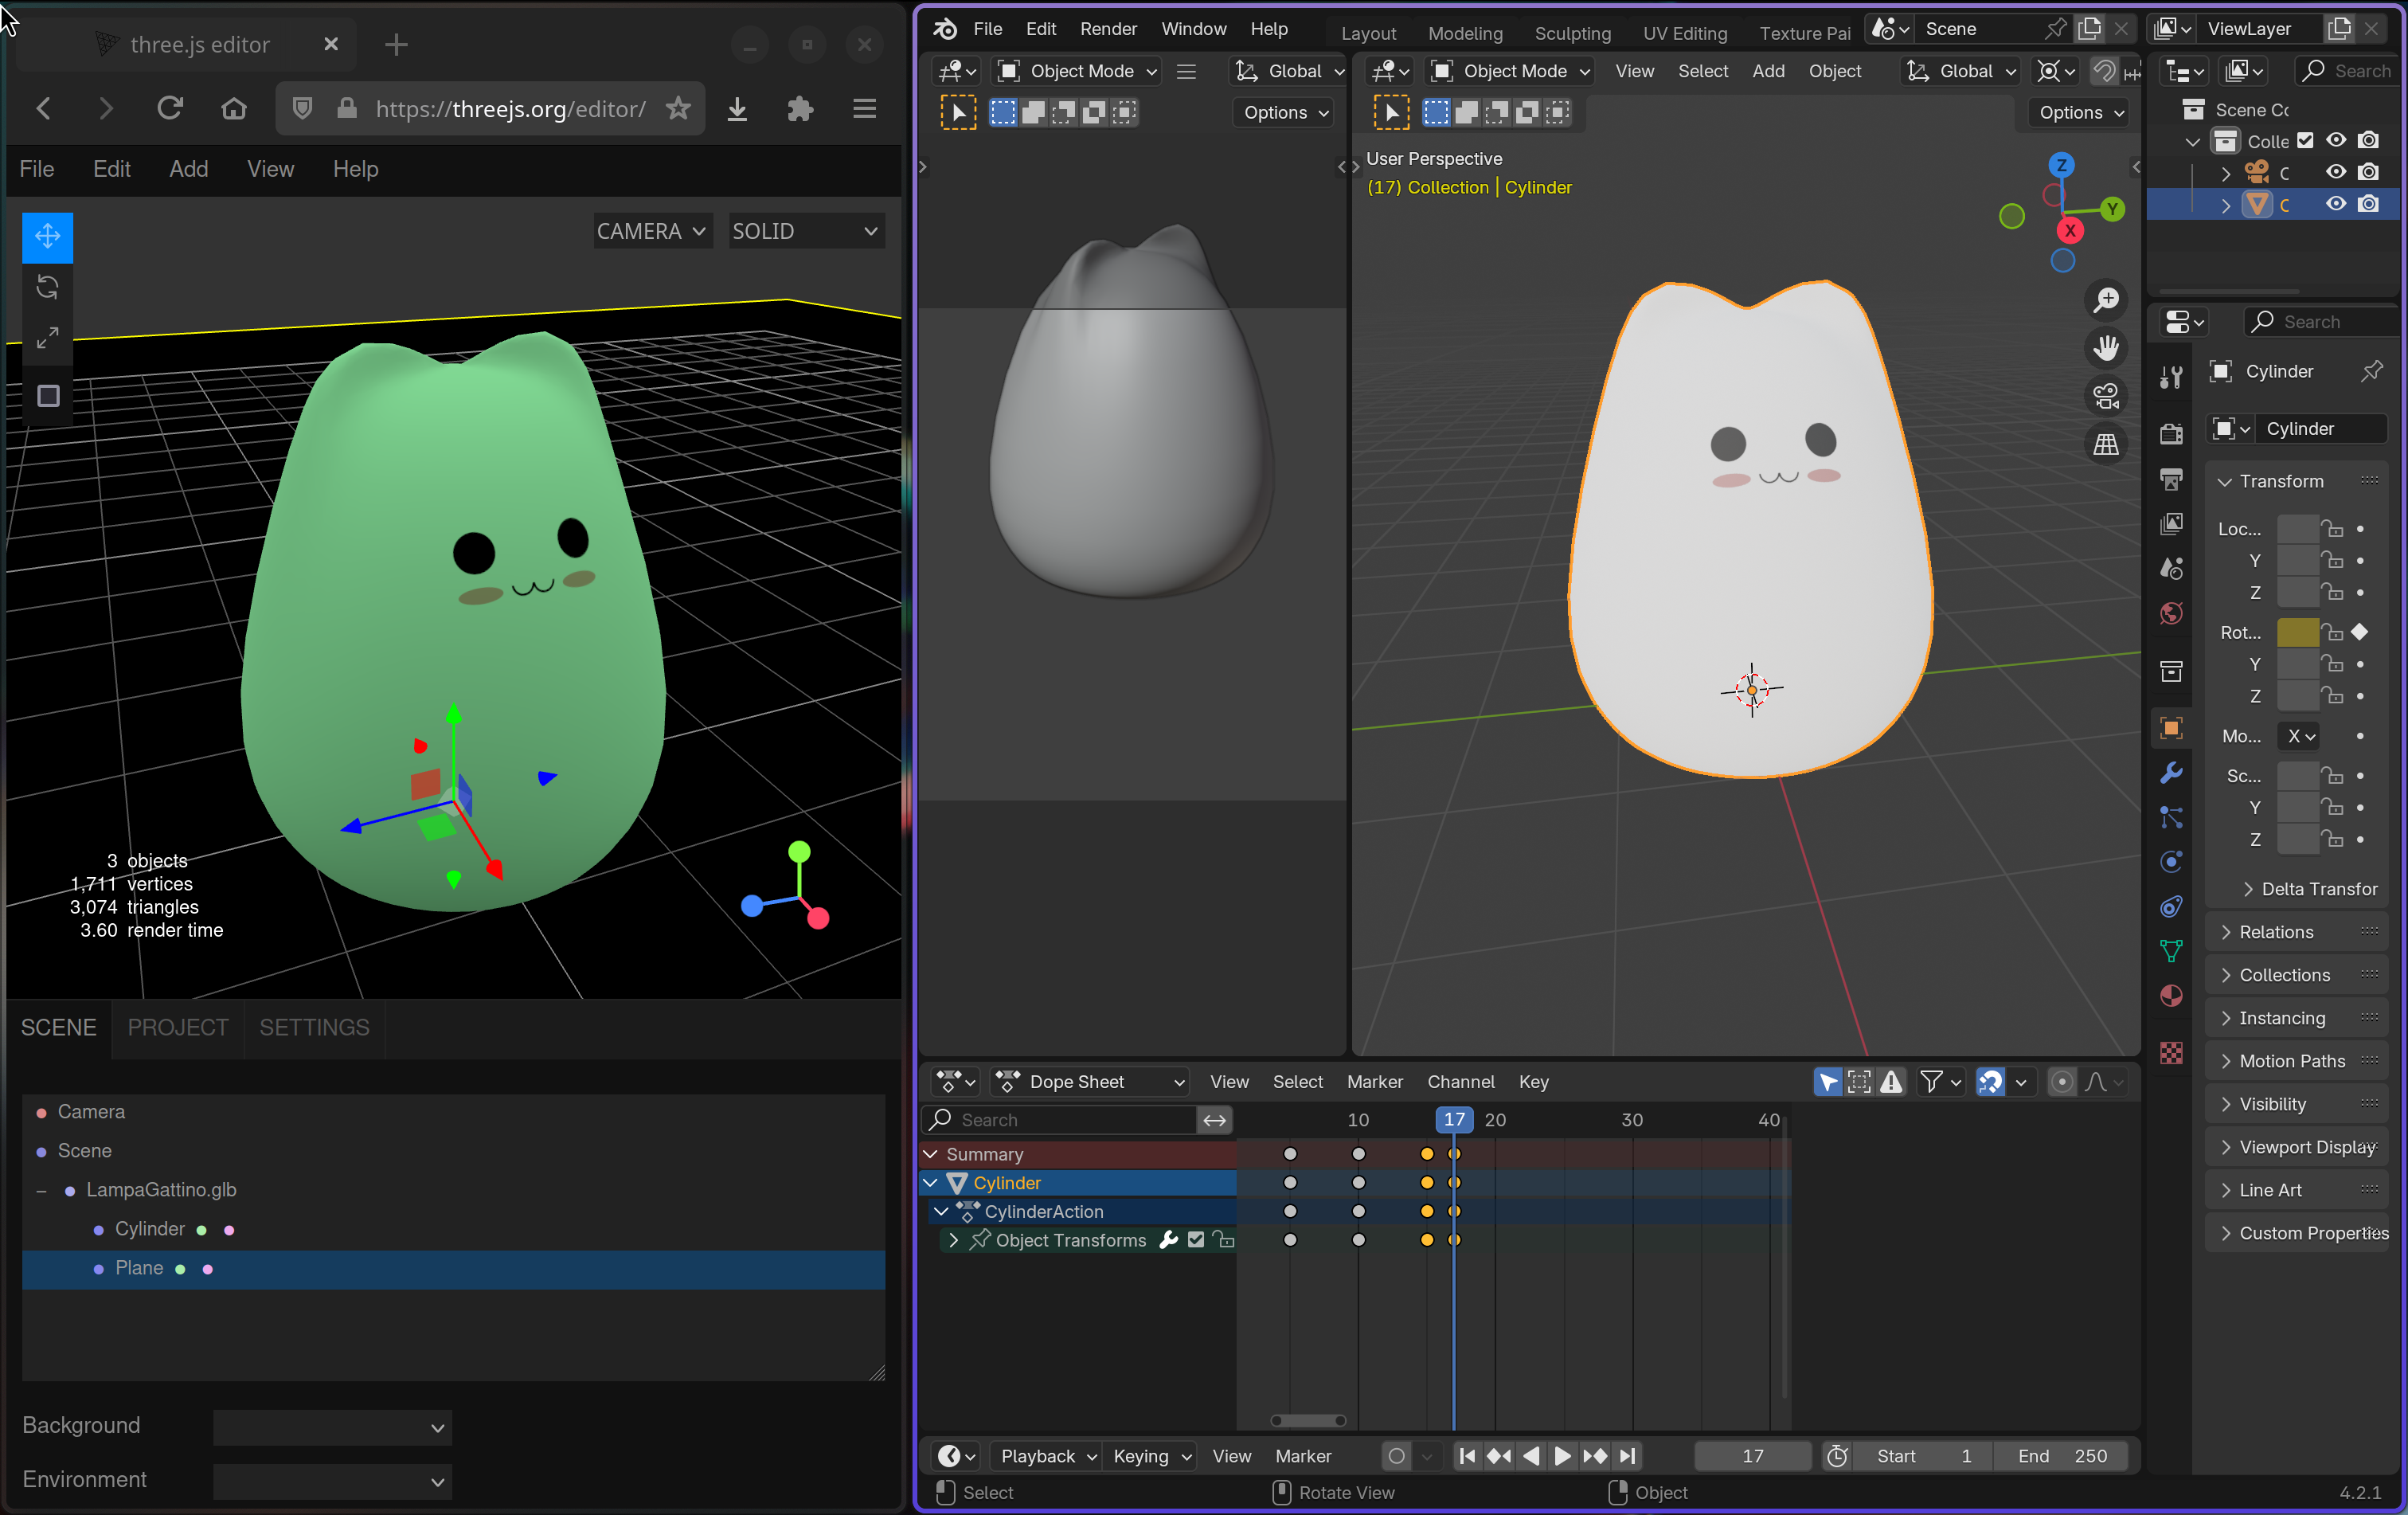
\includegraphics[width=0.8\textwidth]{images/chapter4/blender.png}
    \caption{Modello disegnato su Blender, importato nell'editor Three.js}
    \label{fig:blender}
  \end{figure}

\subsection{WASM}

WebAssembly~\cite{WebAssemblyCoreSpecification1} è uno standard web che definisce un formato binario progettato per essere eseguito all'interno del browser alla 
velocità del codice nativo. 
Linguaggi come Rust, C e C++ possono essere compilati in WebAssembly, permettendo il porting di applicazioni desktop 
sul web senza sacrificarne le prestazioni. 

WASM ha un API che permette al codice JavaScript di comunicare con il codice WebAssembly, rendendo facile l'integrazione
di librerie scritte in Rust all'interno di applicazioni web.

Grazie a WASM è stato possibile emulare i dispositivi direttamente nel browser senza la necessità di installare
software aggiuntivo.

\subsection{WebSocket}

WebSocket è una tecnologia che permette la comunicazione bidirezionale (full-duplex) tra client e server in tempo reale,
mantenendo un canale di comunicazione aperto per inviare e ricevere messaggi senza dover ricorrere 
alla costosa operazione di polling (ovvero la richiesta di aggiornamenti a intervalli regolari).  

Il protocollo WebSocket consente una comunicazione bidirezionale tra un client
e un server, consentendo al server di inviare direttamente messaggi a un client
che ha scelto di ricevere le comunicazioni. Il protocollo viaggia su TCP e consiste in un handshake di apertura
seguito da un framing di base dei messaggi.~\cite{rfc6455}

Essso si è rivelato fondamentale per la comunicazione in tempo reale tra i dispositivi e il server federato, 
così come tra il server e l'emulatore eseguito nel browser. 

\subsection{Sled}

Sled~\cite{sled_website} è un motore di database embedded minimale scritto in Rust, adatto a progetti che richiedono un database
veloce, affidabile e facile da integrare. 

Esso supporta le operazioni ACID (Atomicity, Consistency, Isolation, Durability) e si basa su un algoritmo di B-Tree.

Poiché sled non supporta operazioni su strutture dati complesse, è stato necessario ricorrere alla crate \texttt{typed\_sled}~\cite{typed_sled}
che ha permesso di definire strutture dati custom e di serializzarle e deserializzarle in modo automatico ed ergonomico.

\subsection{Rocket}

Rocket~\cite{rocketrs_website} è un framework web scritto in Rust in grado di creare applicazioni web in modo semplice e veloce.
Esso si basa su un sistema di macro che semplifica la definizione di rotte, middleware e gestione degli errori, 
inoltre gestisce automaticamente la serializzazione e la deserializzazione dei dati in formato JSON e permette di definire rotte
protette da autenticazione.

In aggiunta, tramite il crate rocket\_ws~\cite{rocket_ws} è possibile implementare facilmente la comunicazione WebSocket, feature 
che è stata ampiamente sfruttata in questo progetto.
